\begin{figure}%[htbp]
\centering
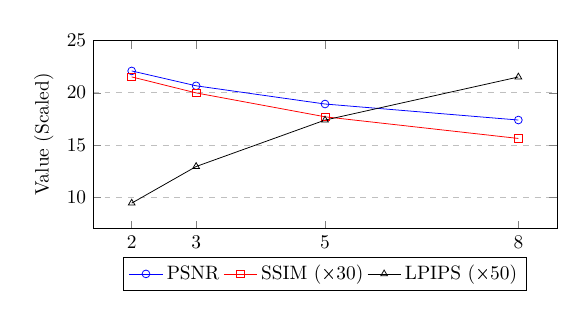
\begin{tikzpicture}[scale=0.7][hbtp]
    \begin{axis}[
        width=10cm,
        height=5cm,
        xlabel={Views},
        ylabel={Value (Scaled)},
        xtick={2,3,5,8},
        ymin=7, ymax=25,
        legend style={
            at={(0.5,-0.15)},
            anchor=north,
            legend columns=-1
        },
        ymajorgrids=true,
        grid style=dashed
    ]
    
    %--- PSNR 原始数据 ---
    \addplot[
        color=blue,
        mark=o
    ]
    coordinates {
        (2,22.08)
        (3,20.66)
        (5,18.920)
        (8,17.39)
    };
    \addlegendentry{PSNR}

    %--- SSIM 数据 (×30) ---
    \addplot[
        color=red,
        mark=square
    ]
    coordinates {
        (2,0.717*30)
        (3,0.666*30)
        (5,0.590*30)
        (8,0.521*30)
    };
    \addlegendentry{SSIM (×30)}

    %--- LPIPS 数据 (×50) ---
    \addplot[
        color=black,
        mark=triangle
    ]
    coordinates {
        (2,0.189*50)
        (3,0.259*50)
        (5,0.3477*50)
        (8,0.430*50)
    };
    \addlegendentry{LPIPS (×50)}
    \end{axis}
\end{tikzpicture}
\caption{\textbf{Relationship between MVSplat Performance and Input Views.}}
\label{view_number}
\end{figure}
